\chapter{Постановка задачи декодирования сигналов}
\label{ch:intro}

В данной главе ставится общая задача декодирования временных рядов.
Приводится обзор стандартных методов анализа временных рядов.
Ставится задача построения оптимальной линейной регрессионной модели декодирования.
Приведен обзор методов снижения размерности пространства, их обобщений и модификаций.

%%%%%%%%%%%%%%%%%%%%%%%%%%%%%%%%%%%%%%%%%%%%%%%%
\section{Регрессионная модель в пространстве высокой размерности}
\label{sec:ch1:reg_model}
%%%%%%%%%%%%%%%%%%%%%%%%%%%%%%%%%%%%%%%%%%%%%%%%

Пусть $\bbX \subset \bbR^n$~--- пространство исходной переменной, $\bbY \subset \bbR^r$~--- пространство целевой переменной.
Пусть задано множество объектов $\{(\bx_i, \by_i)\}_{i=1}^m$, где $\bx_i \in \bbX$~--- исходный объект, $\by_i \in \bbY$~--- целевой объект.

Обозначим за $\bX \in \bbR^{m \times n}$ матрицу исходной переменной, за $\bY \in \bbR^{n \times k}$ матрицу целевой переменной:
\begin{equation*}
	\bX = [\bx_1, \dots, \bx_m]^{\T} =  [\bchi_1, \dots, \bchi_n]; \quad \bY = [\by_1, \dots, \by_m]^{\T} =  [\bnu_1, \dots, \bnu_r].
\end{equation*}

Столбцы~$\{\bchi_j\}_{j=1}^n$ матрицы~$\bX$ являются исходными признаками, столбцы~$\{\bnu_j\}_{j=1}^r$ матрицы~$\bY$ являются целевыми векторами.

Предполагается, что между исходным объектом $\bx$ и целевым объектом $\by$ существует зависимость. Требуется построить прогностическую модель $\mathbf{f}: \bbX \rightarrow \bbY$ из пространства исходной переменной в пространство целевой переменной.

Задача восстановления регрессионной зависимости состоит в нахождении оптимальной модели $\mathbf{f}^*$ по заданным матрицам $\bX$ и $\bY$. Под оптимальностью понимается нахождение такой модели, которая бы доставляла минимум некоторой функции ошибки $\cL$:
\begin{equation}
	\mathbf{f}^* = \argmin_\mathbf{f} \cL(\mathbf{f}, \bX, \bY).
	\label{ch1:eq:loss_min}
\end{equation}

Задача поиска оптимальной модели является задачей функциональной оптимизации. 
Для сужения пространства поиска моделей будем рассматривать параметрические модели $\mathbf{f}(\bx, \bTheta)$, где $\bTheta$~--- \textit{параметры модели}. 
Таким образом между объектами $\bx$ и $\by$ существует зависимость вида
\begin{equation}
	\by = \mathbf{f}(\bx, \bTheta) + \boldsymbol{\varepsilon},
	\label{ch1:eq:reg_model}
\end{equation}
где $\mathbf{f}$~--- параметрическая прогностическая модель, $\bTheta$~--- параметры модели, $\bepsilon \in \bbR^{m}$~--- вектор регрессионных остатков. 

Задача~\eqref{ch1:eq:loss_min} сводится к задаче поиска оптимальных параметров
\begin{equation}
	\bTheta^* = \argmin_{\bTheta} \cL(\bTheta, \bX, \bY).
	\label{ch1:eq:loss_min_param}
\end{equation}

В диссертации рассматривается случай избыточной размерности пространств~$\bbX$, $\bbY$. 
В таком случае решение задачи~\eqref{ch1:eq:loss_min_param} оказывается неустойчивым. 
Рассмотрим в качестве примера задачу восстановления линейной регрессии.

Предположим, что зависимость $\mathbf{f}(\bx, \bTheta)$ линейная:
\begin{equation}
	\by = \mathbf{f}(\bx, \bTheta) + \bepsilon = \bTheta^{\T} \bx+ \bepsilon,
	\label{ch1:eq:lin_reg_model}
\end{equation}
где $\bTheta \in \bbR^{n \times r}$~--- матрица параметров модели.

Оптимальные параметры~$\bTheta$ определяются минимизацией функции ошибки $\cL(\bTheta, \bX, \bY)$.
При решении задачи линейной регрессии в качестве такой функции ошибки рассматривается квадратичная функция потерь:
\begin{equation}
	\cL(\bTheta, \bX, \bY) = {\left\| \underset{m \times r}{\mathbf{Y}}  - \underset{m \times n}{\bX} \cdot \underset{r \times n}{\bTheta} \right\| }_2^2 \rightarrow\min_{\bTheta}.
	\label{ch1:eq:l2_loss_function}
\end{equation}
Решением~\eqref{ch1:eq:l2_loss_function} является следующая матрица:
\begin{equation*}
	\bTheta = (\bX^{\T} \bX)^{-1} \bX^{\T} \bY.
\end{equation*}

Наличие линейной зависимости между столбцами матрицы~$\bX$ приводит к неустойчивому решению задачи оптимизации~\eqref{ch1:eq:l2_loss_function}.
Если существует вектор~$\boldsymbol{\alpha} \neq \bZero_n$ такой, что $\bX \boldsymbol{\alpha}= \bZero_m$, то добавление~$\boldsymbol{\alpha}$ к любому столбцу матрицы~$\bTheta$ не меняет значение функции потерь~$\cL(\bTheta, \bX, \bY)$.
В этом случае матрица~$\bX^{\T} \bX$ близка к сингулярной и не обратима.
Чтобы избежать сильной линейной зависимости между признаками, в данной работе исследуются методы снижения размерности и выбора признаков.

%%%%%%%%%%%%%%%%%%%%%%%%%%%%%%%%%%%%%%%%%%%%%%%%
\section{Задача декодирования сигналов}
\label{sec:ch1:decoding_task}
%%%%%%%%%%%%%%%%%%%%%%%%%%%%%%%%%%%%%%%%%%%%%%%%

Задача декодирования сигналов состоит в восстановлении регрессионной зависимости~\eqref{ch1:eq:loss_min} между наборами гетерогенных сигналов.

Пусть имеется два множества временных рядов $\mathcal{S}_{\bx} = \{\bs_{\bx}^i\}_{i=1}^m$ и $\mathcal{S}_{\by} = \{\bs_{\by}^i\}_{i=1}^r$, состоящие из $m$ и $r$ временных рядов соответственно. 
Первое множество $\mathcal{S}_{\bx}$ является множеством временных рядов $m$ исходных сигналов. 
Второе множество~$\mathcal{S}_{\by}$ является множеством временных рядов $r$ целевых сигналов.
Каждый временной ряд $\bs = (s_1, s_2, \dots, s_T)$ является последовательностью измерений некоторый величины в течение времени. 
\begin{definition}
	 \textit{Временное представление} $\bx_t = ([\bs_{\bx}^1]_t, \dots, [\bs_{\bx}^m]_t) \in \bbR^m$ состоит из измерений временных рядов исходных сигналов в момент времени $t$. 
	Аналогично временное представление $\by_t = ([\bs_{\by}^1]_t, \dots, [\bs_{\by}^r]_t) \in \bbR^r$ состоит из измерений временных рядов целевых сигналов в момент времени $t$.
\end{definition}
\begin{definition}
	Определим \textit{представление предыстории} длины $h$ для момента времени $t$ множества временных рядов исходных сигналов $\mathcal{S}_{\bx}$ как совокупность представлений $\bX_{t,h} = [\bx_{t - h + 1}, \dots, \bx_{t}]^{\T} \in \bbR^{h \times m}$.
	Аналогично определим представление предыстории длины $h$ для момента времени $t$ множества временных рядов целевых сигналов $\mathcal{S}_{\by}$ как совокупность представлений $\bY_{t,h} = [\by_{t - h + 1}, \dots, \by_{t}]^{\T} \in \bbR^{h \times r}$.
\end{definition}
\begin{definition}
	Определим \textit{представление горизонта прогнозирования} длины $p$ для момента времени $t$ множества временных рядов исходных сигналов~$\mathcal{S}_{\bx}$ как совокупность представлений $\bX_{t,p} = [\bx_{t + 1}, \dots, \bx_{t + p}]^{\T} \in \bbR^{p \times m}$.
	Аналогично определим представление горизонта прогнозирования длины $p$ для момента времени $t$ множества временных рядов целевых сигналов $\mathcal{S}_{\by}$ как совокупность представлений $\bY_{t,r} = [\by_{t + 1}, \dots, \by_{t + p}]^{\T} \in \bbR^{p \times r}$.
\end{definition}

Задача авторегрессионного декодирования состоит в построении прогностической модели $\mathbf{f}^{\text{AR}}$, дающей прогноз представления горизонта прогнозирования множества временных рядов по представлению предыстории прогнозирования того же множества временных рядов.

\begin{definition}
	\label{ch1:def:autoreg_model}
	Прогностическая модель $\mathbf{f}^{\text{AR}}_{\bx}: \bbR^{h \times m} \rightarrow \bbR^{p \times m}$ является \textit{авторегрессионной моделью}, которая по представлению предыстории $\bX_{t,h}$ множества временных рядов исходных сигналов $\mathcal{S}_{\bx}$ предсказывает представление горизонта прогнозирования $\bX_{t,p}$ множества временных рядов исходных сигналов $\mathcal{S}_{\bx}$.
	Аналогично вводится прогностическая модель $\mathbf{f}^{\text{AR}}_{\by}: \bbR^{h \times r} \rightarrow \bbR^{p \times r}$ для множества целевых сигналов $\mathcal{S}_{\by}$.
\end{definition}
Суть авторегрессионного декодирования заключается в предсказании будущего прогноза сигнала по его же предыстории.

\begin{definition}
	\label{ch1:def:reg_model}
	Определим задачу \textit{регрессионного декодирования} как задачу построения прогностической модели $\mathbf{f}^{\text{R}}_{\bx\by}: \bbR^{h \times m} \rightarrow \bbR^{p \times r}$, которая по представлению предыстории $\bX_{t,h}$ множества временных рядов исходных сигналов $\mathcal{S}_{\bx}$ предсказывает представление горизонта прогнозирования $\bY_{t,p}$ множества временных рядов целевых сигналов $\mathcal{S}_{\by}$.
\end{definition}

Отличие регрессионного декодирования от авторегрессионного декодирования состоит в том, что в случае регрессионного декодирования представление предыстории и представление горизонта прогнозирования получены из временных рядов разных пространств. 
Предыстория получена из множества исходных сигналов, в то время как горизонт прогнозирования получен из множества целевых сигналов. 
Пространства исходных и целевых сигналов могут являться существенно гетерогенными и обладать разными свойствами.

\begin{definition}
	\label{ch1:def:decode_model}
	Общая \textit{задача декодирования} состоит в построении прогностической модели $\mathbf{f}_{\bx\by}: \bbR^{h_x \times m} \times \bbR^{h_y \times r} \rightarrow \bbR^{p \times r}$, которая по представлениям предыстории $\bX_{t,h_x}$ и $\bY_{t,h_y}$ временных рядов исходных и целевых сигналов предсказывает представление горизонта прогнозирования $\bY_{t,r}$ временных рядов целевых сигналов. 
\end{definition}

Отметим, что авторегрессионная модель $\mathbf{f}^{\text{AR}}_{\by}$ и регрессионная модель $\mathbf{f}^{\text{R}}_{\bx\by}$ являются частными случаями общей задачи декодирования. А именно, авторегрессионная модель $\mathbf{f}^{\text{AR}}_{\by}$ соответствует случаю пустой предыстории временных рядов исходных сигналов (случаю $h_x = 0$), а регрессионная модель $\mathbf{f}^{\text{R}}_{\bx\by}$ соответствует случаю пустой предыстории временных рядов целевых сигналов (случаю $h_y = 0$).

На Рис.~\ref{ch1:fig:time_series_decoding} схематично продемонстрированы принципы построения введенных моделей декодирования временных рядов.

\begin{figure}
	\centering
	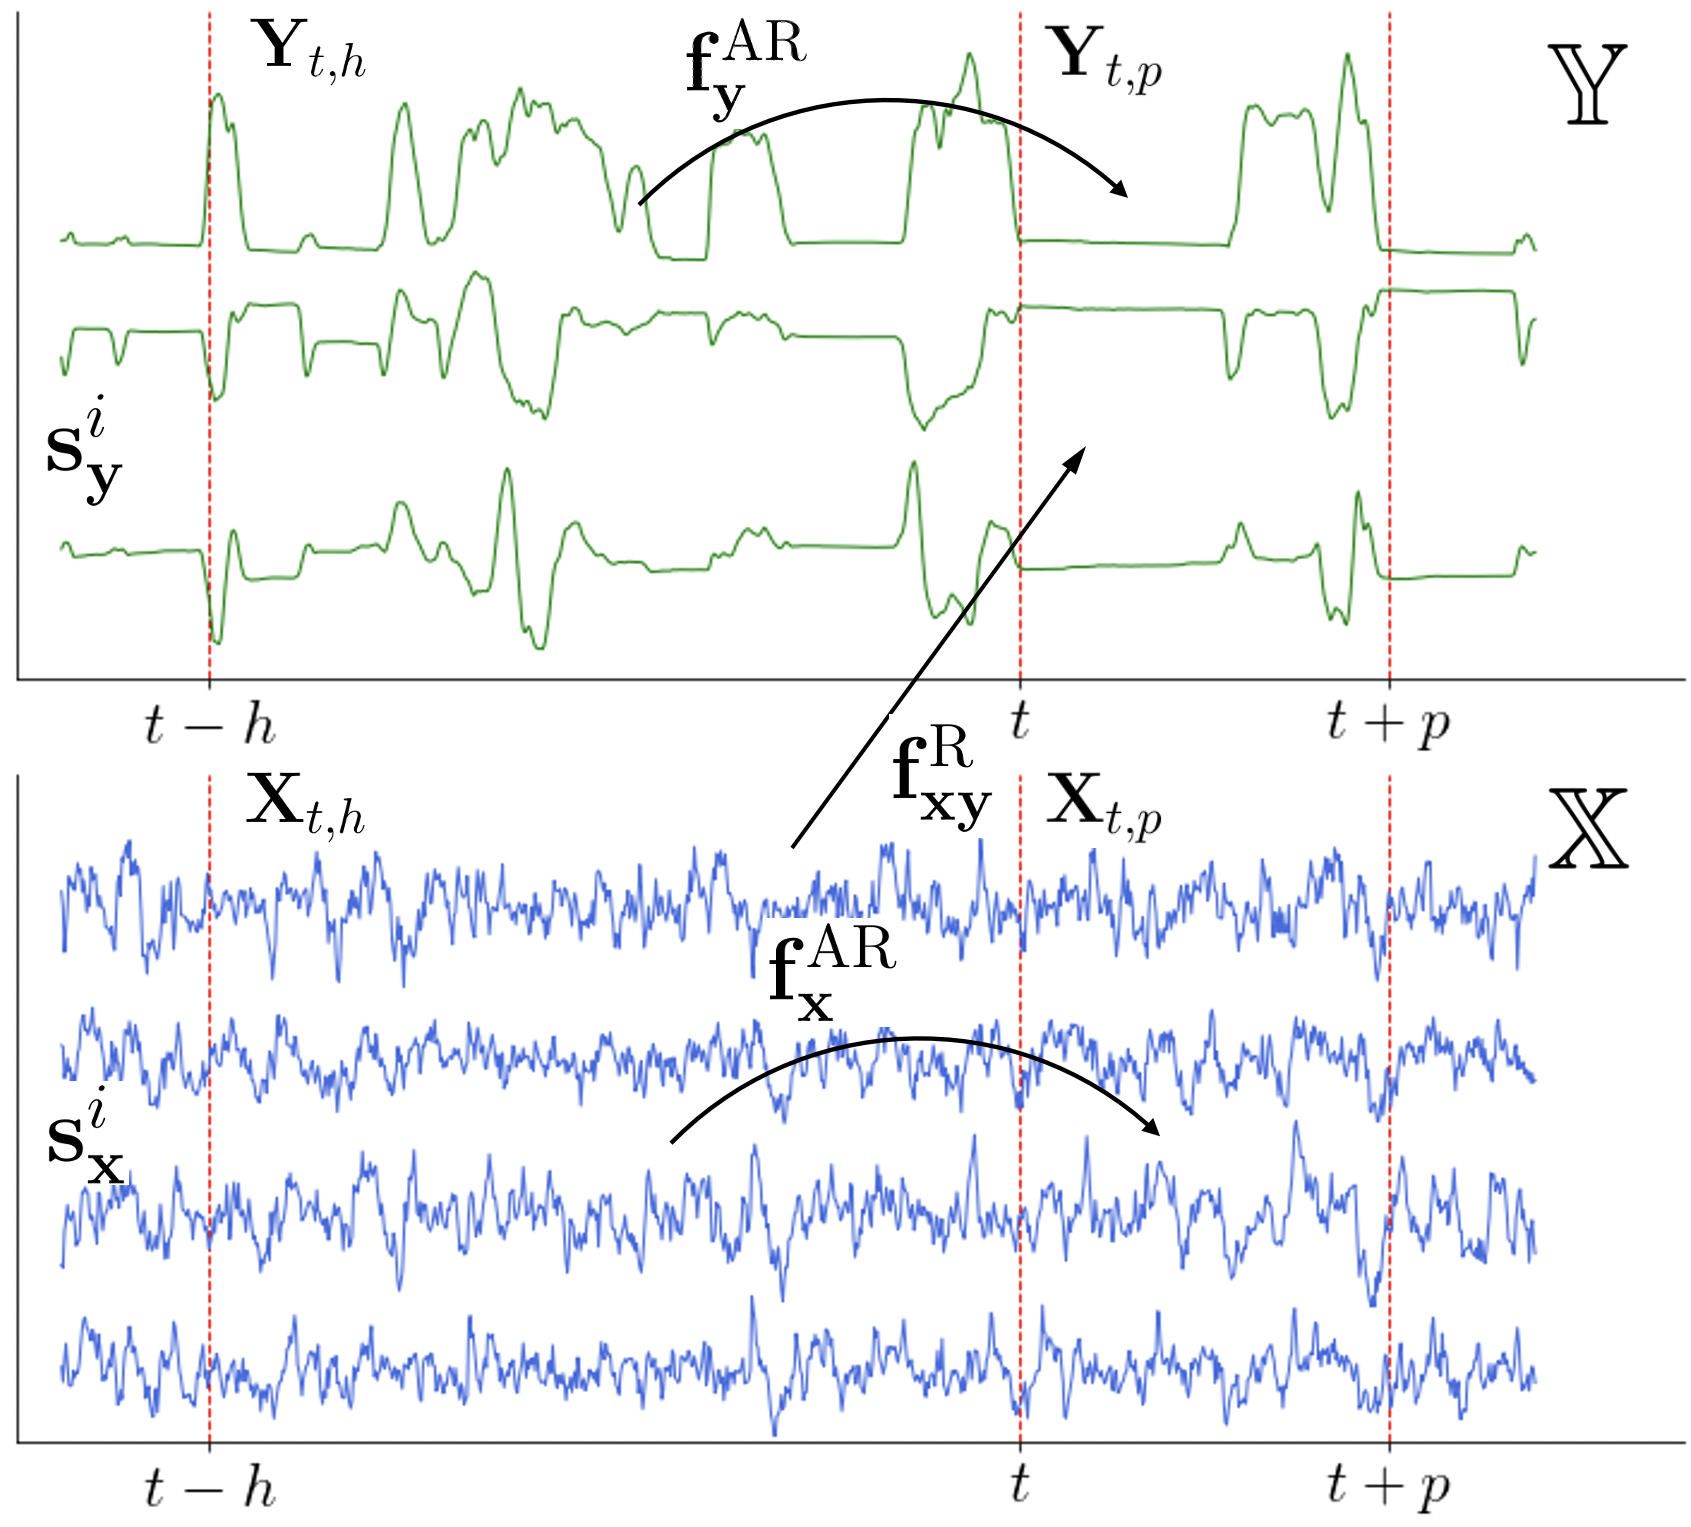
\includegraphics[width=0.7\linewidth]{figs/ch1/time_series_decoding}
	\caption{Схема построения моделей декодирования}
	\label{ch1:fig:time_series_decoding}
\end{figure}

Для построения авторегрессионной модели декодирования временных рядов широко используются два класса линейных методов: авторегрессионные модели и модели скользящего среднего~\cite{box2011time,hipel1994time}. 
Авторегрессионные модели AR($p$) строят прогноз в виде линейной комбинации $p$ предыдущих значений временного ряда.
Модели скользящего среднего MA($q$) вместо предыдущих значений временного ряда используют комбинацию ошибок.
Модель ARMA($p$, $q$)~\cite{cochrane2005time} является комбинацией двух описанных подходов. 
ARMA($p$, $q$) задает модель как линейную комбинацию $p$ предыдущих значений временного ряда и $q$ предыдущих значений ошибок. 
Для нахождения оптимальных параметров $p$ и $q$ модели ARMA используются автокорреляционная и частная автокорреляционная функции. 

Модель ARMA используется для стационарных временных рядов, отвечающим строгим статистическим предположениям. 
На практике встречается огромное количество нестационарных временных рядов подверженных тренду, сезонности или цикличности.
Модель ARIMA($p$, $d$, $q$)~\cite{cochrane2005time} обобщает модель ARMA для случая нестационарных временных рядов.
ARIMA берёт разности порядка $d$ от исходного временного ряда для достижения стационарности данных. 
При этом на практике оказывается достаточным положить $d = 1$.
Заметим, что при $d = 0$ модель ARIMA эквивалентна модели ARMA. 
Полезным обобщением модели ARIMA является модель AFRIMA~\cite{galbraith2001autoregression}. 
Модель позволяет задать параметр $d$ в виде вещественного числа.

Модель ARIMA плохо справляется с сезонными временными рядами.
В работе~\cite{box2011time} была предложена модель SARIMA, которая вводит в модель учет сезонной компоненты.

Задача декодирования временных рядов декомпозируется на следующие подзадачи.
\begin{itemize}
	\item Порождение признакового пространства. 
	Данный этап включает в себя процедуру извлечения признаков из исходных значений сигналов. 
	Процедура порождения признакового пространства может быть основана на экспертных знаниях или же являться моделью машинного обучения. 
	Данная подзадача подробно рассмотрена в главе~\ref{ch:metamodels}.
	
	\item Снижение размерности пространства или выбор признаков. 
	Исходные временные ряды, а также порожденное признаковое пространство оказывается избыточным, что приводит к избыточности и неустойчивости модели. 
	Методы снижения размерности и выбора признаков подробно изложены в главах~\ref{ch:pls} и~\ref{ch:qpfs}.
	
	\item Построение модели.
	После нахождения оптимального низкоразмерного представления исходных данных ставится задача выбора оптимальной модели декодирования.
\end{itemize}

%%%%%%%%%%%%%%%%%%%%%%%%%%%%%%%%%%%%%%%%%%%%%%%%
\section{Обзор методов снижения размерности для задачи декодирования}
\label{sec:ch1:dim_reduction}
%%%%%%%%%%%%%%%%%%%%%%%%%%%%%%%%%%%%%%%%%%%%%%%%
Методы снижения размерности позволяют найти низкоразмерное представление исходных данных. 
Найденное представление используется для построения прогностической модели.
При этом метод снижения размерности может учитывать как зависимости в исходном объекте~$\bx$, так и в целевом объекте~$\by$.

\subsubsection{Метод главных компонент для задачи декодирования.}
Для устранения линейной зависимости и снижения размерности исходного пространства объектов широко используется метод главных компонент~(principal component analysis, PCA). 
Метод PCA находит низкоразмерное представление матрицы~$\bX = \bT \bP$, такое что новое представление~$\bT \in \bbR^{m \times l}$ содержит максимальную долю дисперсии исходной матрицы.
При этом матрица отображения $\bP \in \bbR^{l \times n}$ ($\bP \bP^{\T} = \bI$) содержит правые собственные вектора матрицы ковариаций $\bX^{\T} \bX$.

Метод PCA является базовым методом снижения размерности пространства. 
Существует множество модификаций базового метода.
Bероятностный PCA~\cite{tipping1999probabilisticpca} рассматривает задачу снижения размерности в терминах вероятностной модели, решая задачу с помощью вариационного EM алгоритма. 
Разреженный PCA~\cite{zou2006sparsepca} вводит в постановку задачи lasso регуляризацию для того, чтобы сделать матрицу отображения~$\bP$ разреженной и более интерпретируемой.
Нелинейный ядерный PCA~\cite{scholkopf1997kernelpca} отображает исходные данные с помощью нелинейного отображения и использует RKHS для решения исходной задачи.

После нахождения матрицы отображения $\bP$ задача~\eqref{ch1:eq:l2_loss_function} принимает вид
\begin{equation}
	\cL(\bB, \bT, \bY) = {\left\| \underset{m \times r}{\mathbf{Y}}  - \underset{m \times l}{\bT} \cdot \underset{l \times r}{\bB} \right\| }_2^2 \rightarrow\min_{\bB}.
	\label{ch1:eq:l2_loss_function_pca}
\end{equation}

Модель прогнозирования~\eqref{ch1:eq:lin_reg_model} в случае снижения размерности с помощью PCA принимает вид:
\begin{equation}
	\by = \bB^{\T} \bt + \bepsilon = \bB^{\T} \bP \bx + \bepsilon = \bTheta \bx + \bepsilon, \, \text{ где } \bTheta = \bB^{\T} \bP.
	\label{ch1:eq:lin_reg_model_pca}
\end{equation}

\subsubsection{Метод частичных наименьших квадратов для задачи декодирования.}
Основным недостатком метода PCA является отсутствие учёта взаимосвязи между исходными признаками~$\bchi_j$ и целевыми векторами~$\bnu_j$.
Метод частичных наименьших квадратов (partial least squares, PLS) проецирует матрицу исходных объектов~$\bX$ и матрицу целевых объектов в скрытое пространство малой размерностью~$l$ ($l < n$).
Метод PLS находит в скрытом пространстве матрицы~$\bT, \bU \in \bbR^{m \times l}$, которые лучше всего описывают исходные матрицы~$\bX$ и~$\bY$. 
При этом PLS максимизирует ковариацию между столбцами матриц $\bT$ и $\bU$ соответственно.
Принцип работы метода показан на следующей коммутативной диаграмме:
\begin{equation}
		\begin{tikzpicture}
			\matrix (m) [matrix of math nodes,row sep=3em,column sep=2em,minimum width=2em,ampersand replacement=\&]
			{
				\bx \in \bbR^n \& \& \by \in \bbR^r \\
				\& \bt, \bu \in \bbR^\ell \& \\};
			\path[-stealth]
			(m-1-1) edge node [above] {$\mathbf{f}$} (m-1-3)
			(m-1-1) edge [bend right=10] node [below, pos=0.4] {$\bW$} (m-2-2)
			(m-2-2) edge [bend right=10] node [above, pos=0.4] {$\bP$} (m-1-1)
			(m-1-3) edge [bend left=10] node [below, pos=0.4] {$\bC$} (m-2-2)
			(m-2-2) edge [bend left=10] node [above, pos=0.4] {$\bQ$} (m-1-3);
		\end{tikzpicture}
\end{equation}

Метод PLS был впервые предложен в работах~\cite{wold1975path,wold1984collinearity,wold1982pls}. Подробное описание алгоритма приведено в работах~\cite{geladi1986partial,geladi1988notes,de1993simpls,vinzi2010handbook,brereton2014partial}.
В работах~\cite{rosipal2005overview,rosipal2011nonlinear} приведен обзор обобщений базовой модели PLS.
В работе~\cite{chun2010sparse} приведена модификация метода PLS для получения разреженного набора признаков. 
 
Матрица исходных объектов $\bX$ и матрица целевых объектов $\bY$ проецируются на скрытое пространство следующим образом:
\begin{align}
	\label{ch1:eq:PLS_X}
	\underset{m \times n}{\bX} 
	&= \underset{m \times l}{\bT} \cdot \underset{l \times n}{\bP} + \underset{m \times n}{\bE_{\bx}} 
	= \sum_{k=1}^l \underset{m \times 1}{\btau_k} \cdot \underset{1 \times n}{\bp_k^{\T}} + \underset{m \times n}{\bE_{\bx}},\\
	\label{ch1:eq:PLS_Y}
	\underset{m \times r}{\bY} 
	&= \underset{m \times l}{\bU} \cdot \underset{l \times r}{\bQ} + \underset{m \times r}{\bE_{\by}}
	=  \sum_{k=1}^l  \underset{m \times 1}{\bnu_k} \cdot \underset{1 \times r}{\bq_k^{\T}} +  \underset{m \times r}{\bE_{\by}}.
\end{align}
Здесь $\bT$ и $\bU$~--- образы исходных матриц в скрытом пространстве, причём столбцы матрицы $\bT$ ортогональны; $\bP$ и $\bQ$~--- матрицы перехода; $\bE_{\bx}$ и $\bE_{\by}$~--- матрицы остатков. 
Метод PLS восстанавливает линейную зависимость между столбцами матриц~$\bT$ и~$\bU$
\begin{equation*}
	\bU \approx \bT \bB, \quad \bB = \text{diag}(\beta_k), \quad \beta_k = \bnu_k^{\T}\btau_k / (\btau_k^{\T}\btau_k),
\end{equation*}
где $\{\btau_k\}_{k=1}^l$, $\{\bnu_k\}_{k=1}^l$~--- столбцы матриц $\bT$ и $\bU$ соответственно.

Метод решает следующую оптимизационную задачу:
\begin{equation}
	\max_{\|\bp\|_{2}=\|\bq\|_{2}=1}[ \text{cov}(\bX \bp, \bY \bq)^{2}] = \max_{\bp, \bq} \frac{\bp^{\T} \bX^{\T} \bY \bq}{\sqrt{\bp^{\T} \bp} \sqrt{\bq^{\T} \bq}}.
	\label{ch1:eq:pls_max_cov}
\end{equation}
Детальное описание алгоритма работы метода PLS с доказательством его корректности приведено в разделе~\ref{sec:ch2:pls_proof}.

Для демонстрации разницы между методами PCA и PLS был проведен модельный эксперимент для случая, когда размерности пространств исходных объектов, целевых объектов и скрытого пространства равны 2 ($n = r = l = 2$).
Исходные объекты~$\bx_i$ сгенерированы из нормального распределения с нулевым матожиданием. 
Целевые объекты~$\by_i$ линейным образом зависят от второй  главной компоненты $pc_2$ матрицы $\bX$ и не зависят от первой главной компоненты $pc_1$.
На Рис.~\ref{ch1:fig:pls_toy_example} показаны результаты работы методов. 
Синими и зелёными точками изображены исходные объекты~$\bx_i$ и целевые объекты~$\by_i$. 
Красным контуром показаны линии уровня матриц ковариаций распределений. 
Черным изображены единичные окружности. 
Красные стрелки соответствуют главным компонентам матриц~$\bX$ и~$\bY$. 
Черные стрелки соответствуют векторам матриц~$\bW$ и~$\bC$ метода PLS. 
Данные матрицы содержат вектора, являющиеся аналогами главных компонент метода PCA.
Учёт взаимной связи между матрицами~$\bX$ и~$\bY$ отклоняет вектора~$\bw_k$ и~$\bc_k$ от направления главных компонент. 
\begin{figure}[h]
	\centering
	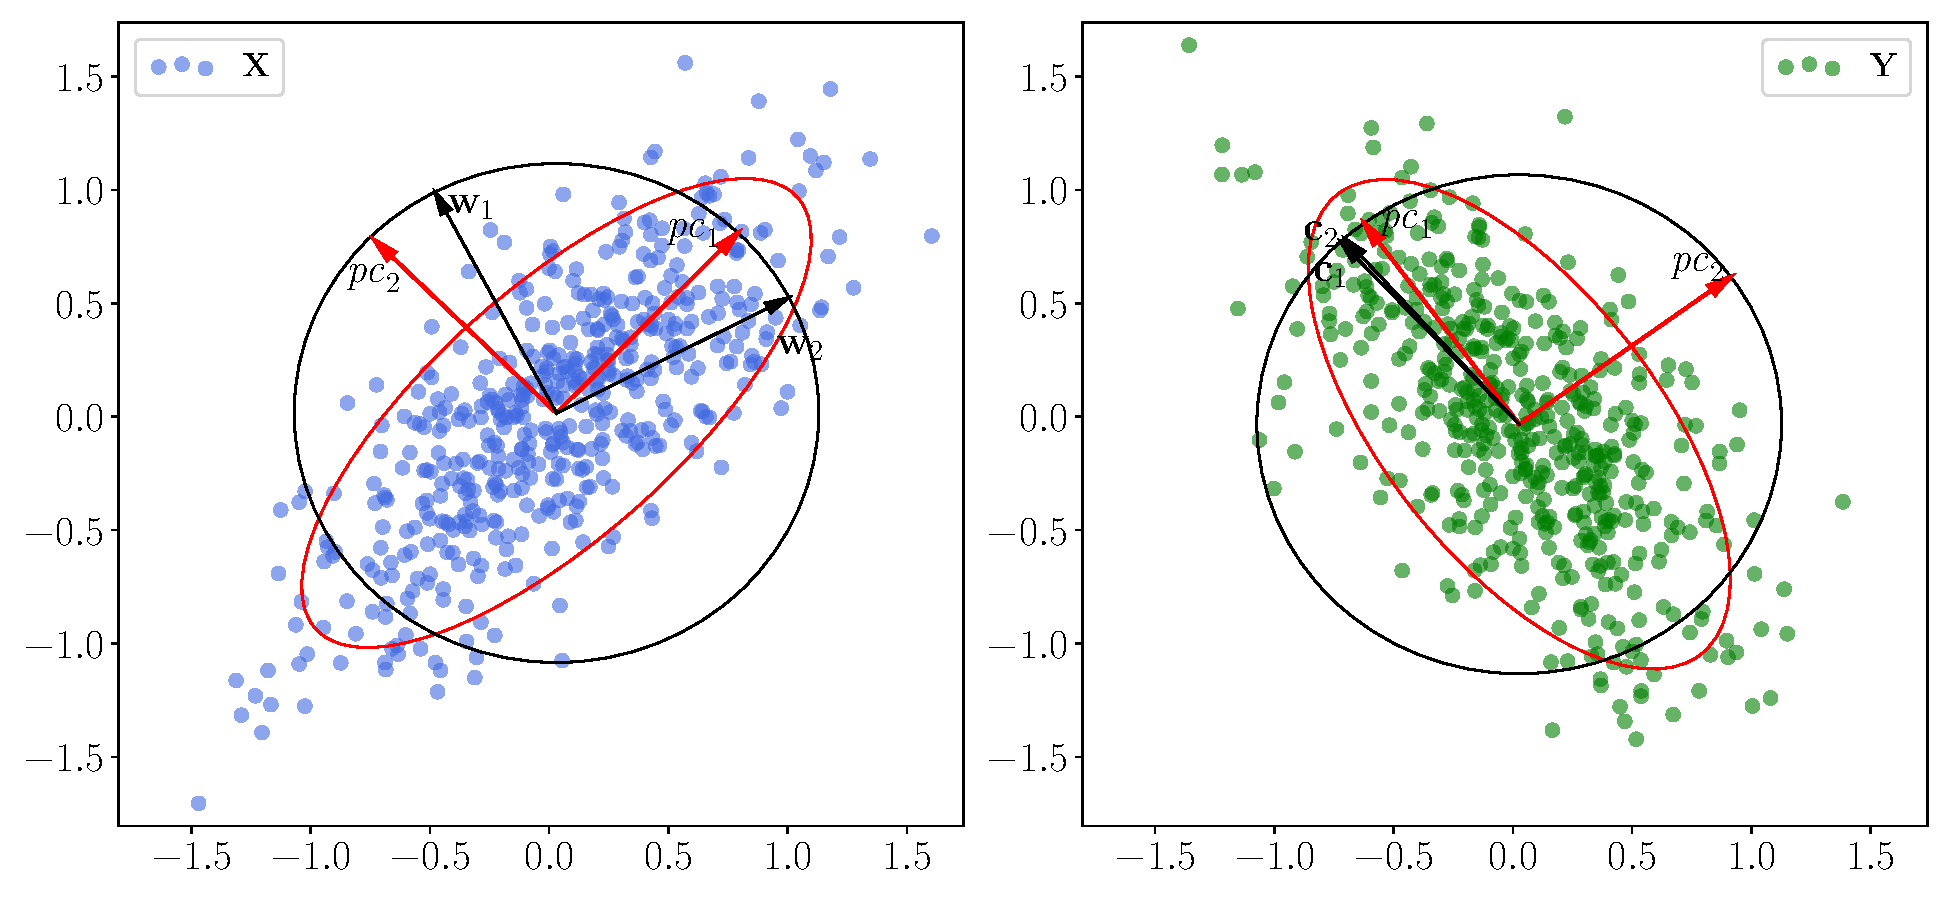
\includegraphics[width=\linewidth]{figs/ch1/pls_toy_example}
	\caption{Модельный пример работы методов PCA и PLS}
	\label{ch1:fig:pls_toy_example}
\end{figure}

При снижении размерности пространств до одного признака метод PCA выберет первую главную компоненту $pc_1$, отбросив компоненту $pc_2$, так как первая компонента объясняет большую часть дисперсии исходной матрицы $\bX$. 
При этом матрица $\bY$ не зависит от $pc_1$. 
Тем самым финальная модель окажется не адекватной.
Метод PLS позволяет побороться с данной проблемой.

\subsubsection{Канонический анализ корреляций для задачи декодирования.}
Канонический корреляционный анализ (canonical correlation analysis, CCA) широко применяется для поиска взаимосвязи между двумя наборами переменных~\cite{hotelling1992relations,anderson1962introduction}. 
Оптимизационная задача CCA похожа на оптимизационную задачу PLS~\eqref{ch1:eq:pls_max_cov} с той лишь разницей, что вместо максимизации ковариации CCA максимизирует корреляцию:
\begin{equation}
	\max_{\|\bp\|_{2}=\|\bq\|_{2}=1}[ \text{corr}(\bX \bp, \bY \bq)^{2}] = \max_{\bp, \bq} \frac{\bp^{\T} \bX^{\T} \bY \bq}{\sqrt{\bp^{\T} \bX^{\T}  \bX \bp} \sqrt{\bq^{\T} \bY^{\T}  \bY\bq}}.
	\label{ch1:eq:cca_max_corr}
\end{equation}

На Рис.~\ref{ch1:fig:cca_toy_example} показан результат работы метода. 
Основное различие состоит в том, что вектора $\bc_1$ и $\bc_2$ в данном случае становятся ортогональными.

\begin{figure}[h]
	\centering
	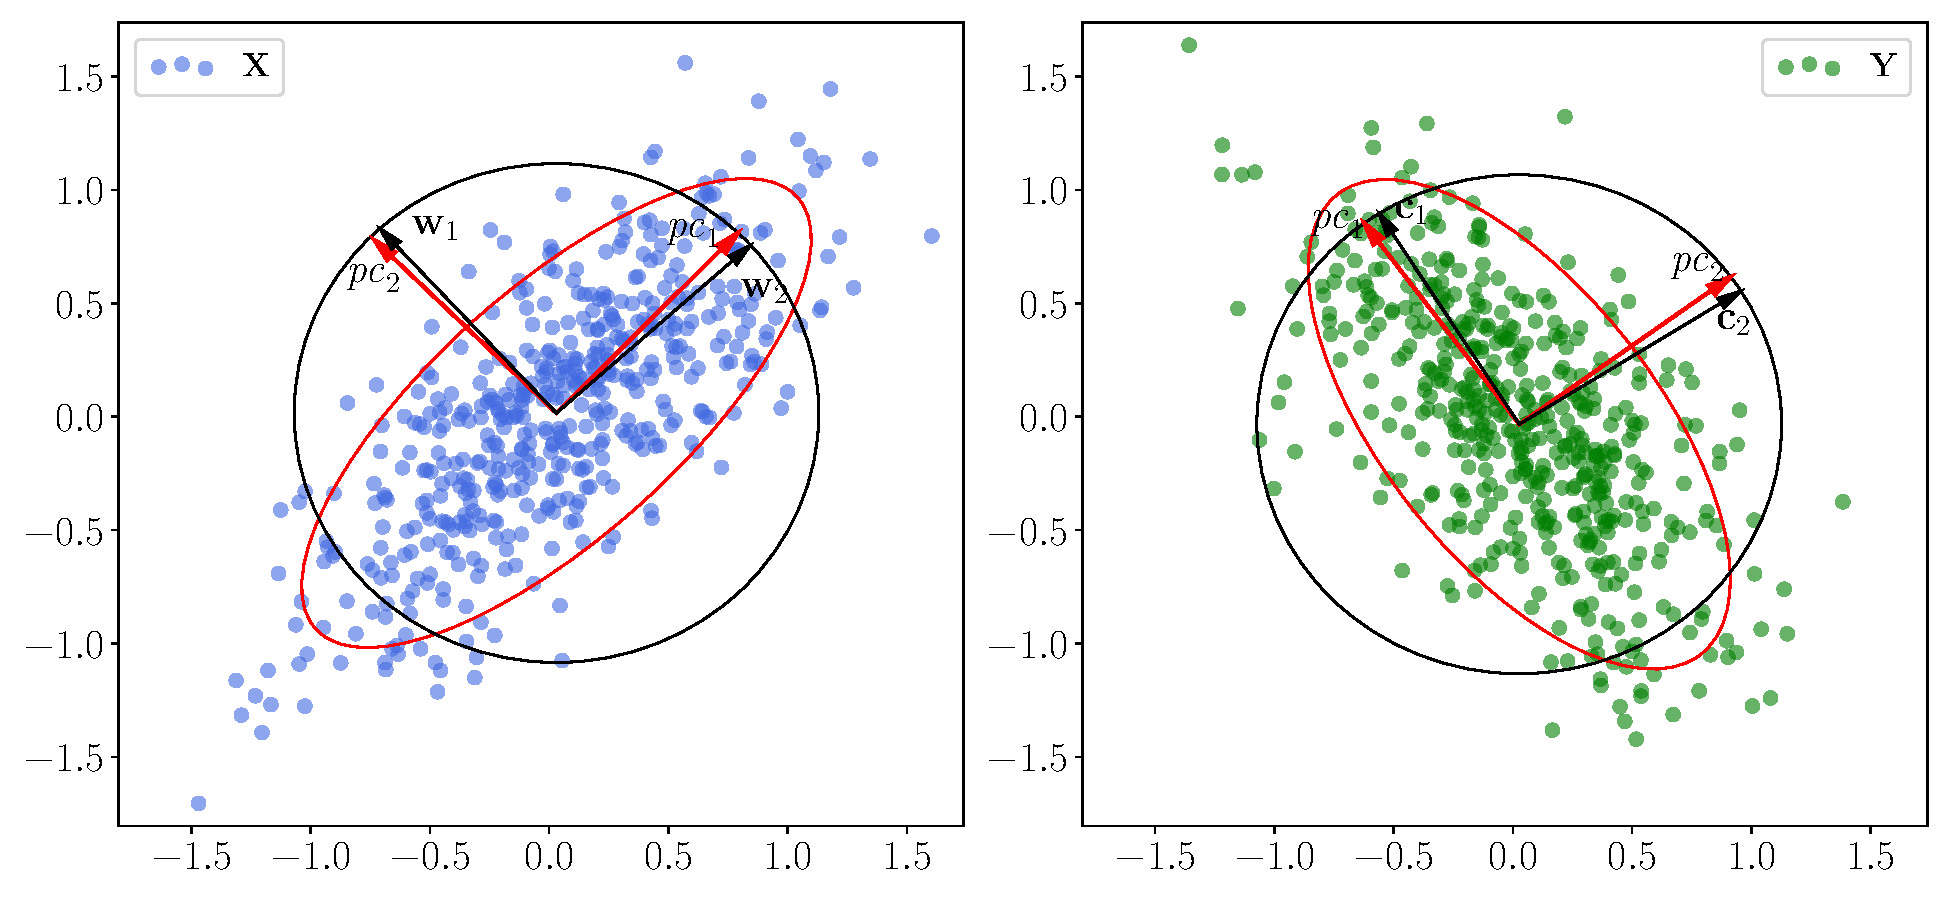
\includegraphics[width=\linewidth]{figs/ch1/cca_toy_example}
	\caption{Модельный пример работы методов PCA и CCA}
	\label{ch1:fig:cca_toy_example}
\end{figure}

В таблице~\ref{ch1:tbl:toy_example_results} приведены значения квадратичной ошибки $\mathcal{L}(\bTheta, \bX, \bY)$ для методов линейной регрессии, PCA, PLS и CCA.
Линейная регрессия отлично справляется с данной задачей.
Ошибка метода PCA наибольшая, что подтверждает факт, что для данной ситуации метод не находит нужных зависимостей в пространстве целевой переменной. 
Методы PLS и CCA показывают схожие результаты.

\begin{table}[]
	\centering
	\begin{tabular}{|c|c|c|c|}
		\hline
		\textbf{Линейная регрессия} & \textbf{PCA}   & \textbf{PLS}  &  \textbf{CCA}  \\ \hline
		0.01 &  0.24   &  0.13 &  0.13 \\ \hline
	\end{tabular}
	\caption{Средняя квадратичная ошибка на модельном примере для методов линейной регрессии, PCA, PLS, CCA}
	\label{ch1:tbl:toy_example_results}
\end{table} 

Нелинейный ядерный CCA~\cite{akaho2006kernel,melzer2001nonlinear,bach2002kernel,hardoon2004canonical} является обобщением базового метода. 
CCA и ядерный CCA широко используются для задач обучения без учителя~\cite{hardoon2007unsupervised,vinokourov2003inferring}. 
Метод имеет область применения от анализа хемометрических~\cite{montanarella1995chemometric} и биологических~\cite{vert2003graph} данных до обработки естественного языка~\cite{haghighi2008learning,dhillon2011multi}, аудиосигналов~\cite{choukri1986adaptation,rudzicz2010adaptive} и компьютерного зрения~\cite{kim2007tensor}.

В работе~\cite{andrew2013deep} впервые было предложено обобщение метода CCA, работающего с нейросетями. 
Предложенный метод DeepCCA максимизирует корреляцию между представлениями, полученными на выходе нейросети:
\begin{multline}
	\max_{\|\bp\|_{2}=\|\bq\|_{2}=1}\left[ \text{corr}(\mathbf{G}_{\bx}(\bX, \bW_{\bx}) \cdot \bp, \mathbf{G}_{\by}(\bY, \bW_{\by}) \cdot \bq)^{2}\right] = \\ = \max_{\bp, \bq} \frac{\bp^{\T} \mathbf{G}_{\bx}(\bX, \bW_{\bx})^{\T} \mathbf{G}_{\by}(\bY, \bW_{\by}) \bq}{\sqrt{\bp^{\T} \mathbf{G}_{\bx}(\bX, \bW_{\bx})^{\T}  \mathbf{G}_{\bx}(\bX, \bW_{\bx}) \bp} \sqrt{\bq^{\T} \mathbf{G}_{\by}(\bY, \bW_{\by})^{\T}  \mathbf{G}_{\by}(\bY, \bW_{\by}) \bq}}.
	\label{ch1:eq:depp_cca_max_corr}
\end{multline}
Здесь $\mathbf{G}_{\bx}(\bX, \bW_{\bx})$ и $\mathbf{G}_{\by}(\bY, \bW_{\by})$~--- нелинейные проекции исходных и целевых объектов.
В статье~\cite{wang2015deep} приведен обширный обзор модификаций нейросетевого CCA для работы с многовидовыми данными.
С использованием нейросетевых функций модель декодирования способна учитывать существенно нелинейные зависимости как в исходном пространстве, так и в целевом пространстве.
Главным недостатком нейросетевого CCA является вычислительная сложность. 
В работе~\cite{chang2018scalable} предложена релаксация исходной функции потерь, которая масштабируется для работы с глубокими моделями нейросетей.

\vspace{0.5cm}
\textbf{Тензорные линейные методы для задачи декодирования.}
Если исходный объект $\bx$ является не вектором, а тензором более высокого порядка, то для построения модели тензор может быть вытянут в вектор~\cite{cichocki2009nonnegative}. 
В таком случае модель не учитывает имеющиеся зависимости между различными направлениями исходного тензора.
Для учета таких зависимостей используются тензорные версии метода PLS~\cite{zhao2012higher,eliseyev2013recursive,eliseyev2016penalized}.


\vspace{0.5cm}
\textbf{Многомодальные данные в задаче декодирования.}
Исходный объект может иметь несколько модальностей. 
Примерами таких модальностей могут быть выровненные аудио и видео~\cite{kidron2005pixels,chaudhuri2009multi}, аудио и артикуляция~\cite{arora2012kernel}, изображение и текстовая аннотация~\cite{hardoon2004canonical,socher2010connecting,hodosh2013framing}, параллельный корпус текстов~\cite{vinokourov2003inferring,haghighi2008learning,ap2014autoencoder,faruqui2014improving}.

Если для каждого объекта имеется более двух модальностей, то для построения скрытого пространства применяются два класса подходов. 
Первый подход состоит в построении скрытого пространства для каждой пары модальностей объекта~\cite{masci2013multimodal,rajendran2015bridge}. 
Второй же подход состоит в построении общего единого скрытого пространства для всех модальностей~\cite{kumar2011co,sharma2012generalized}.